\documentclass[a4paper, 12pt]{article}
\usepackage{mathtools}
\usepackage{amssymb}
\usepackage[]{graphicx}
\usepackage[]{hyperref}
\usepackage{hanging}
\usepackage{pgfplots}
\usepackage{siunitx}
\usepackage[margin=1.0in]{geometry}
\usepackage{setspace}
\pgfplotsset{compat=1.7}

\title{The frequency response of the \textit{MXR® MICRO AMP} amplifier}
\author{Marko Vejnovi\'{c}}

\begin{document}
\pagenumbering{gobble}
\maketitle

\section{Introduction}
\paragraph*{}
Frequency response, ie. how flat the graph of the ratio of the amplified 
signal and the input signal is, plays a great role in how good an amplifier is. 
Being interested in both music and electronics, my decision as to what I'd do 
for my physics internal assessment was clear - I'd measure the frequency 
response of an amplifier.
\paragraph*{}
Frequency response is a measure of how much a certain circuit alters the 
amplitude of an input sine signal with respect to the frequency of the signal 
(Horowitz, and Hill). A flat frequency response is one where the output signal 
is amplified by a constant value, independent of the frequency of the input 
signal. Usually, alteration of the frequency response is done with passive 
filters. Even amplifiers that advertise themselves as flat use some sort of 
filter to reduce noise or potential harmonic effects. The derivation for 
the \textit{cutoff frequency}\footnote{Defined as the frequency at which the 
amplitude of a signal is reduced by $3\si{dB}$, ie. the frequency at which the 
power of the signal is approximately halved by a passive first stage filter.} 
is given in the following paragraph.

\paragraph*{} 
Suppose a capacitor is driven by a voltage source with a sinewave frequency 
$V(t) = V_0 sin(\omega t)$. The current of the capacitor is given by:
$$I(t) = C \frac{dV}{dt} = C \omega V_0 cos (\omega t) = 
C \omega V_0 sin(wt + \frac{\pi}{2})$$
This means that the current amplitude is $C \omega V_0$ and that it is offset 
by $\ang{90}$ with respect to the driving voltage. The amplitude (disregarding 
phases) of the current is:
$$I = C \omega V = \frac{V}{1 / (\omega C)}$$
Given that $\omega = 2 \pi f$, it follows that:
$$I = \frac{V}{1 /(2 \pi f C)}$$
$$\frac{I}{V} = 2 \pi f C$$
$$R = \frac{1}{2 \pi f C}$$
Finally:
\begin{equation} 
	f = \frac{1}{2 \pi R C}
	\label{eqn:cutoff-freq}
\end{equation}

\paragraph*{}
Whether an $RC$ circuit is going to be a low-pass one or a high-pass one 
depends on the layout of the circuit. If the capacitor is connected to ground 
it passes the low frequencies (under the cutoff frequency), otherwise, if the 
resistor is connected to ground, the filter passes through higher frequencies.

\paragraph*{}
The \textit{MXR® MICRO AMP} (Jim Dunlop) is a small  $+26\si{dB}$ guitar 
amplifier pedal, based on the \textit{TL061} (Texas Instruments) operational 
amplifier. It is designed specifically not to change the tone of the guitar, 
but instead to provide a clean, boosted signal. Its main application is to 
have louder guitar solos, or to use it when using two guitars of unequal 
output signal power (Jim Dunlop). Note that this is not a guitar amplifier in 
the sense that it is directly connected to a speaker, but rather a 
``stompbox''\footnote{A term for guitar pedals} that increases the voltage of 
the input signal, without increasing the power of the signal. It is impossible 
to directly attach this amplifier to a cabinet\footnote{A technical term which 
represents what can be thought of as a guitar speaker}.

\paragraph*{}
The schematic of the \textit{MXR® MICRO AMP} is given in figure 
\ref{fig:mxr_schematic}.
\begin{figure}[ht] 
	\centering
	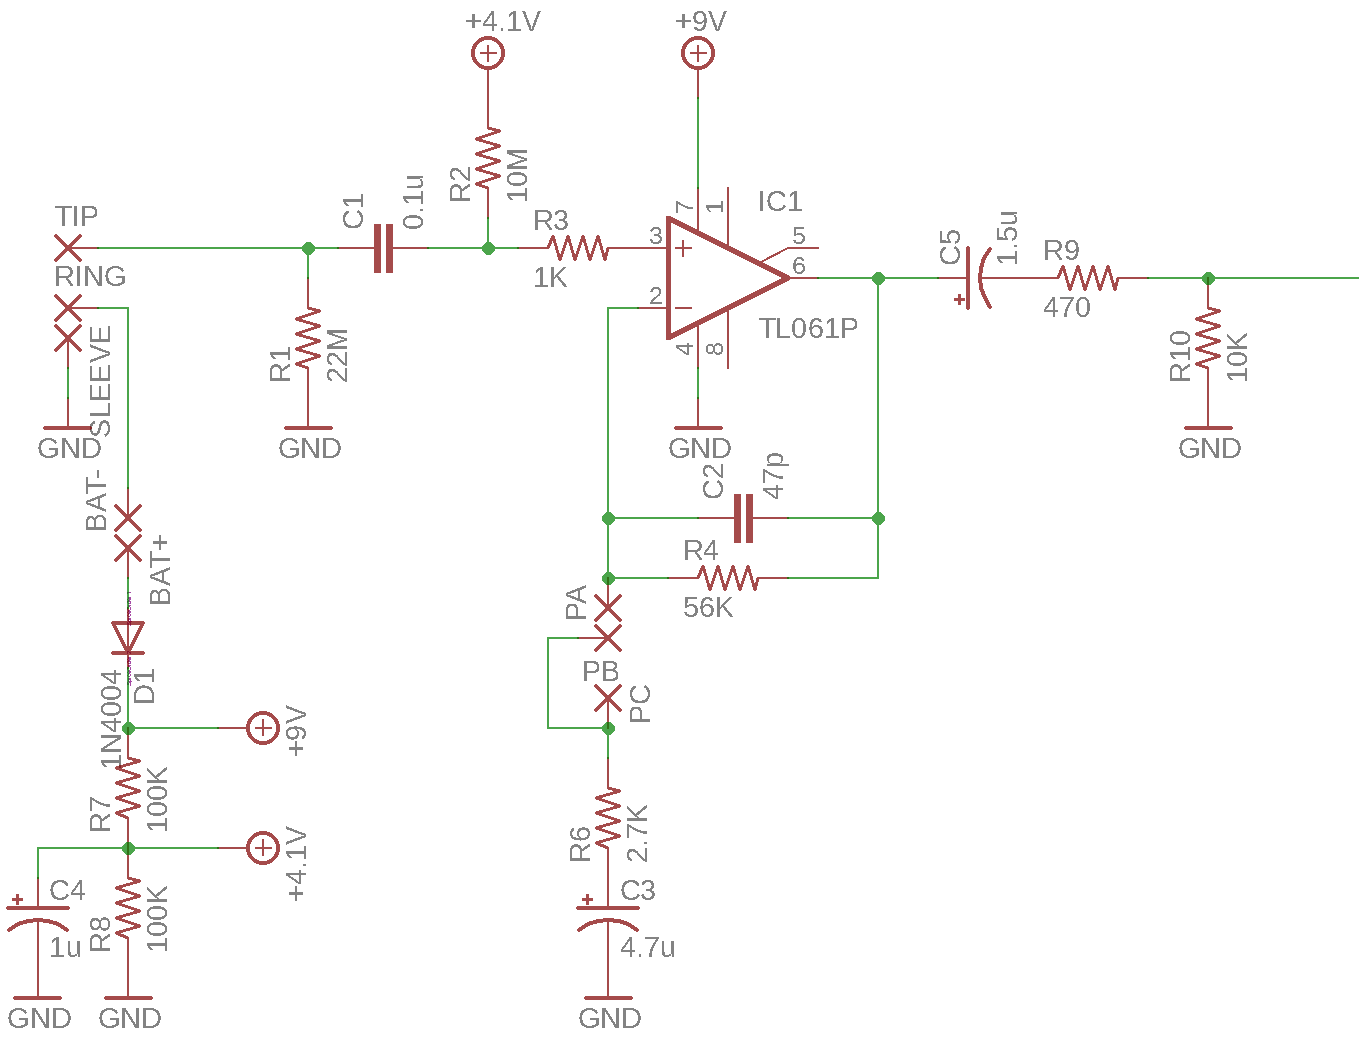
\includegraphics{img/mxr-schematic}
	\caption{The schematic of the \textit{MXR® MICRO AMP}}
	\label{fig:mxr_schematic}
\end{figure}

\paragraph*{}
The circuit is composed out of two major sections - the power regulation 
section and the actual amplifier circuit, both given in figures 
\ref{fig:mxr-power} and \ref{fig:mxr-amp}, respectively.

\begin{figure}[ht]
	\centering
	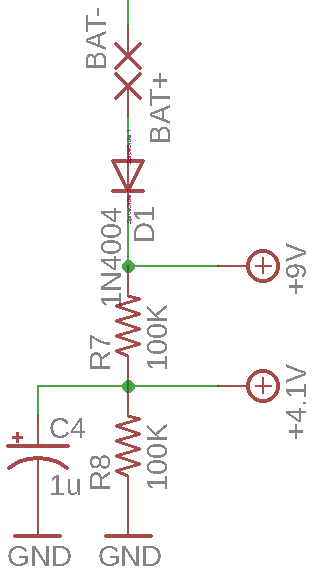
\includegraphics{img/mxr-power}
	\caption{The power regulation section of the \textit{MXR® MICRO AMP}}
	\label{fig:mxr-power}
\end{figure}

\paragraph*{}
The power regulation section is quite simple. It consists out of a rectifier 
diode to protect the circuit from reverse polarity, a low current voltage 
divider ($R_8$ and $R_7$) for stepping down the $+9\si{V}$ DC voltage into 
$+4.5\si{V}$ for use in the amplifier section and a small ceramic capacitor 
($C_4$) for absorbing potential voltage spikes or drops.

\begin{figure}[ht]
	\centering
	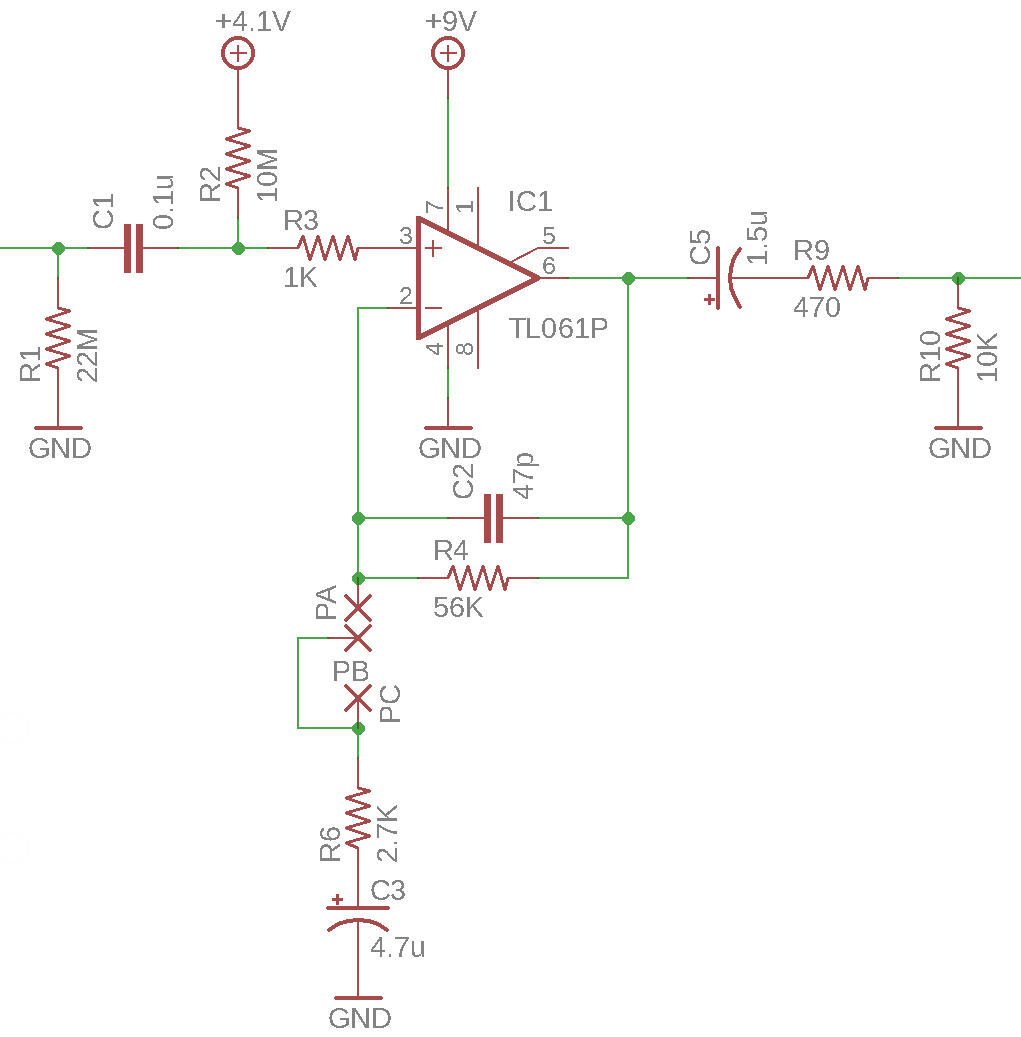
\includegraphics{img/mxr-amp}
	\caption{The amplifier section of the \textit{MXR® MICRO AMP}}
	\label{fig:mxr-amp}
\end{figure}

\paragraph*{}
The amplification section is centered around the $TL061$ operational 
amplifier. $R_1$ is a pull-down resistor which serves as as a method of 
discharging any residual charge that may have built up in $C_1$, in order to 
remove any potential ``popping'' sounds during the connection of the pedal. 
$C_1$ is a coupling capacitor which removes any DC bias. Through $R_2$, the 
signal is offset by $+4.5\si{V}$ because the $TL061$ in this configuration 
only allows for positive amplification. Offsetting the signal by $+4.5\si{V}$ 
allows for bipolar amplification. $C_5$ couples the signal at the output.

\paragraph*{}
$R_4$, $P$\footnote{$P$ is actually supposed to be a $500K\si{\ohm}$ 
potentiometer, but inside the actual pedal the printed circuit board is 
connected via cables to the potentiometer, so in this schematic pad symbols 
($P_A$, $P_B$ and $P_C$) were used.} and $R_6$ control the gain of the $TL061$. 
Since the $TL061$, like any other operational amplifier, tends to make the 
voltage difference between the inputs equal to $0$, and draws negligible 
current (Horowitz, and Hill). Its theoretical gain can be calculated as 
follows. The op-amp\footnote{Operational amplifier} tends to make:
\begin{equation}
	V_{TL061-3} = V_{TL061-2}
	\label{eqn:op-amp-gr-1}
\end{equation}
$R_4$, $P$ and $R_6$ are setup in a manner such that they constitute a voltage 
divider, therefore:
$$V_{TL061-2} = V_{TL061-6} \cdot \frac{P + R_6}{P + R_4 + R_6}$$
Let us define $V_{TL061-6}$ as $V_{out1}$ and $V_{TL061-3}$ as $V_{in}$. Given 
this and from equation \ref{eqn:op-amp-gr-1}, it follows that:
$$V_{in1} = V_{out} \cdot \frac{P + R_6}{P + R_4 + R_6}$$
The gain $G_1$ is then:
$$G_1 = 1 + \frac{R_4}{P + R_6}$$
However, the resistors $R_9$ and $R_{10}$ behave as another voltage divider, 
making the final gain $G$ between the input and the output of the pedal:
$$G = (1 + \frac{R_4}{P + R_6}) \cdot \frac{R_{10}}{R_9 + R_{10}}$$
For the values of the resistors used in the pedal, these calculate to:
$$G_{min} |_{P = 500k\si{\ohm}} = 1.06 \approx 1$$
$$G_{max} |_{P = 0k\si{\ohm}} = 20.8$$

\paragraph*{}
$C_1$, $R_3$ and the $TLP061$ input impedance\footnote{Given in the $TL061$ 
datasheet (Texas Instruments).} together build a high-pass filter, whose 
cutoff frequency is calculated using equation \ref{eqn:cutoff-freq}:
$$f_{C_1} = \frac{1}{2 \pi C_1 (R_2 / (R_3 + Z_{TL061-3})} = 1.59 \si{Hz}$$
It is obvious that this filtering has no effect on the audio, since the 
frequency is inaudible.

\paragraph*{}
$C_2$, together with $R_4$, serves to filter out high harmonics that are 
inaudible, but do introduce noise to the op-amp, potentially over-saturating 
it:
$$f_{C_2} = \frac{1}{2 \pi C_2 R_4} = 60.4\si{kHz}$$

\paragraph*{}
$C_3$ is a very common capacitor used in similar guitar pedals. It is used to 
filter out deep sounds that may saturate the operational amplifier, but are 
inaudible.
$$f_{C_3} = \frac{1}{2 \pi C_3 (P + R_6)}$$
$$f_{C_3 min} |_{P = 500\si{k\ohm}} = 6.74 \cdot 10^{-2} \si{Hz}$$
$$f_{C_3 max} |_{P = 0\si{k\ohm}} = 12.5 \si{Hz}$$

$C_5$ constitutes a very common high-pass filter in similar stompbox designs. 
$R_{10}$ and $C_5$ create a high-pass filter, whose cutoff frequency is:
$$f_{C_5} = \frac{1}{2 \pi C_5 R_{10}} = 10.6 \si{Hz}$$

\paragraph*{}
This amplifier pedal advertises itself as having a flat frequency response. 
The research goal of this paper is to determine the frequency response of the 
pedal. Other studies have determined that the frequency response is, indeed, 
flat (``MXR Microamp Analysis'').

\section{Hypothesis}
\paragraph*{}
It was expected of this pedal to have a flat frequency response and no effects 
on the input signal.

\section{Method}

\paragraph*{}
A copy of the \textit{MXR® MICRO AMP} was assembled on a 
breadboard\footnote{A board which allows for making prototypes of electronic 
circuits easily}. Due to a lack of components, some were substituded. A 
schematic with the used components is given in \ref{fig:mxr-microamp-used}. 
The original $R_1$ is replaced with two resistors that add up to 
$20\si{M\ohm}$, making a small difference between the original $22\si{M\ohm}$. 
$C_5$ was replaced with two $1\si{\micro F}$ capacitors in parallel, bringing 
the cutoff frequency to:
$$f_{C_5} = 7.95 \si{Hz}$$
\begin{figure}[ht]
	\centering
	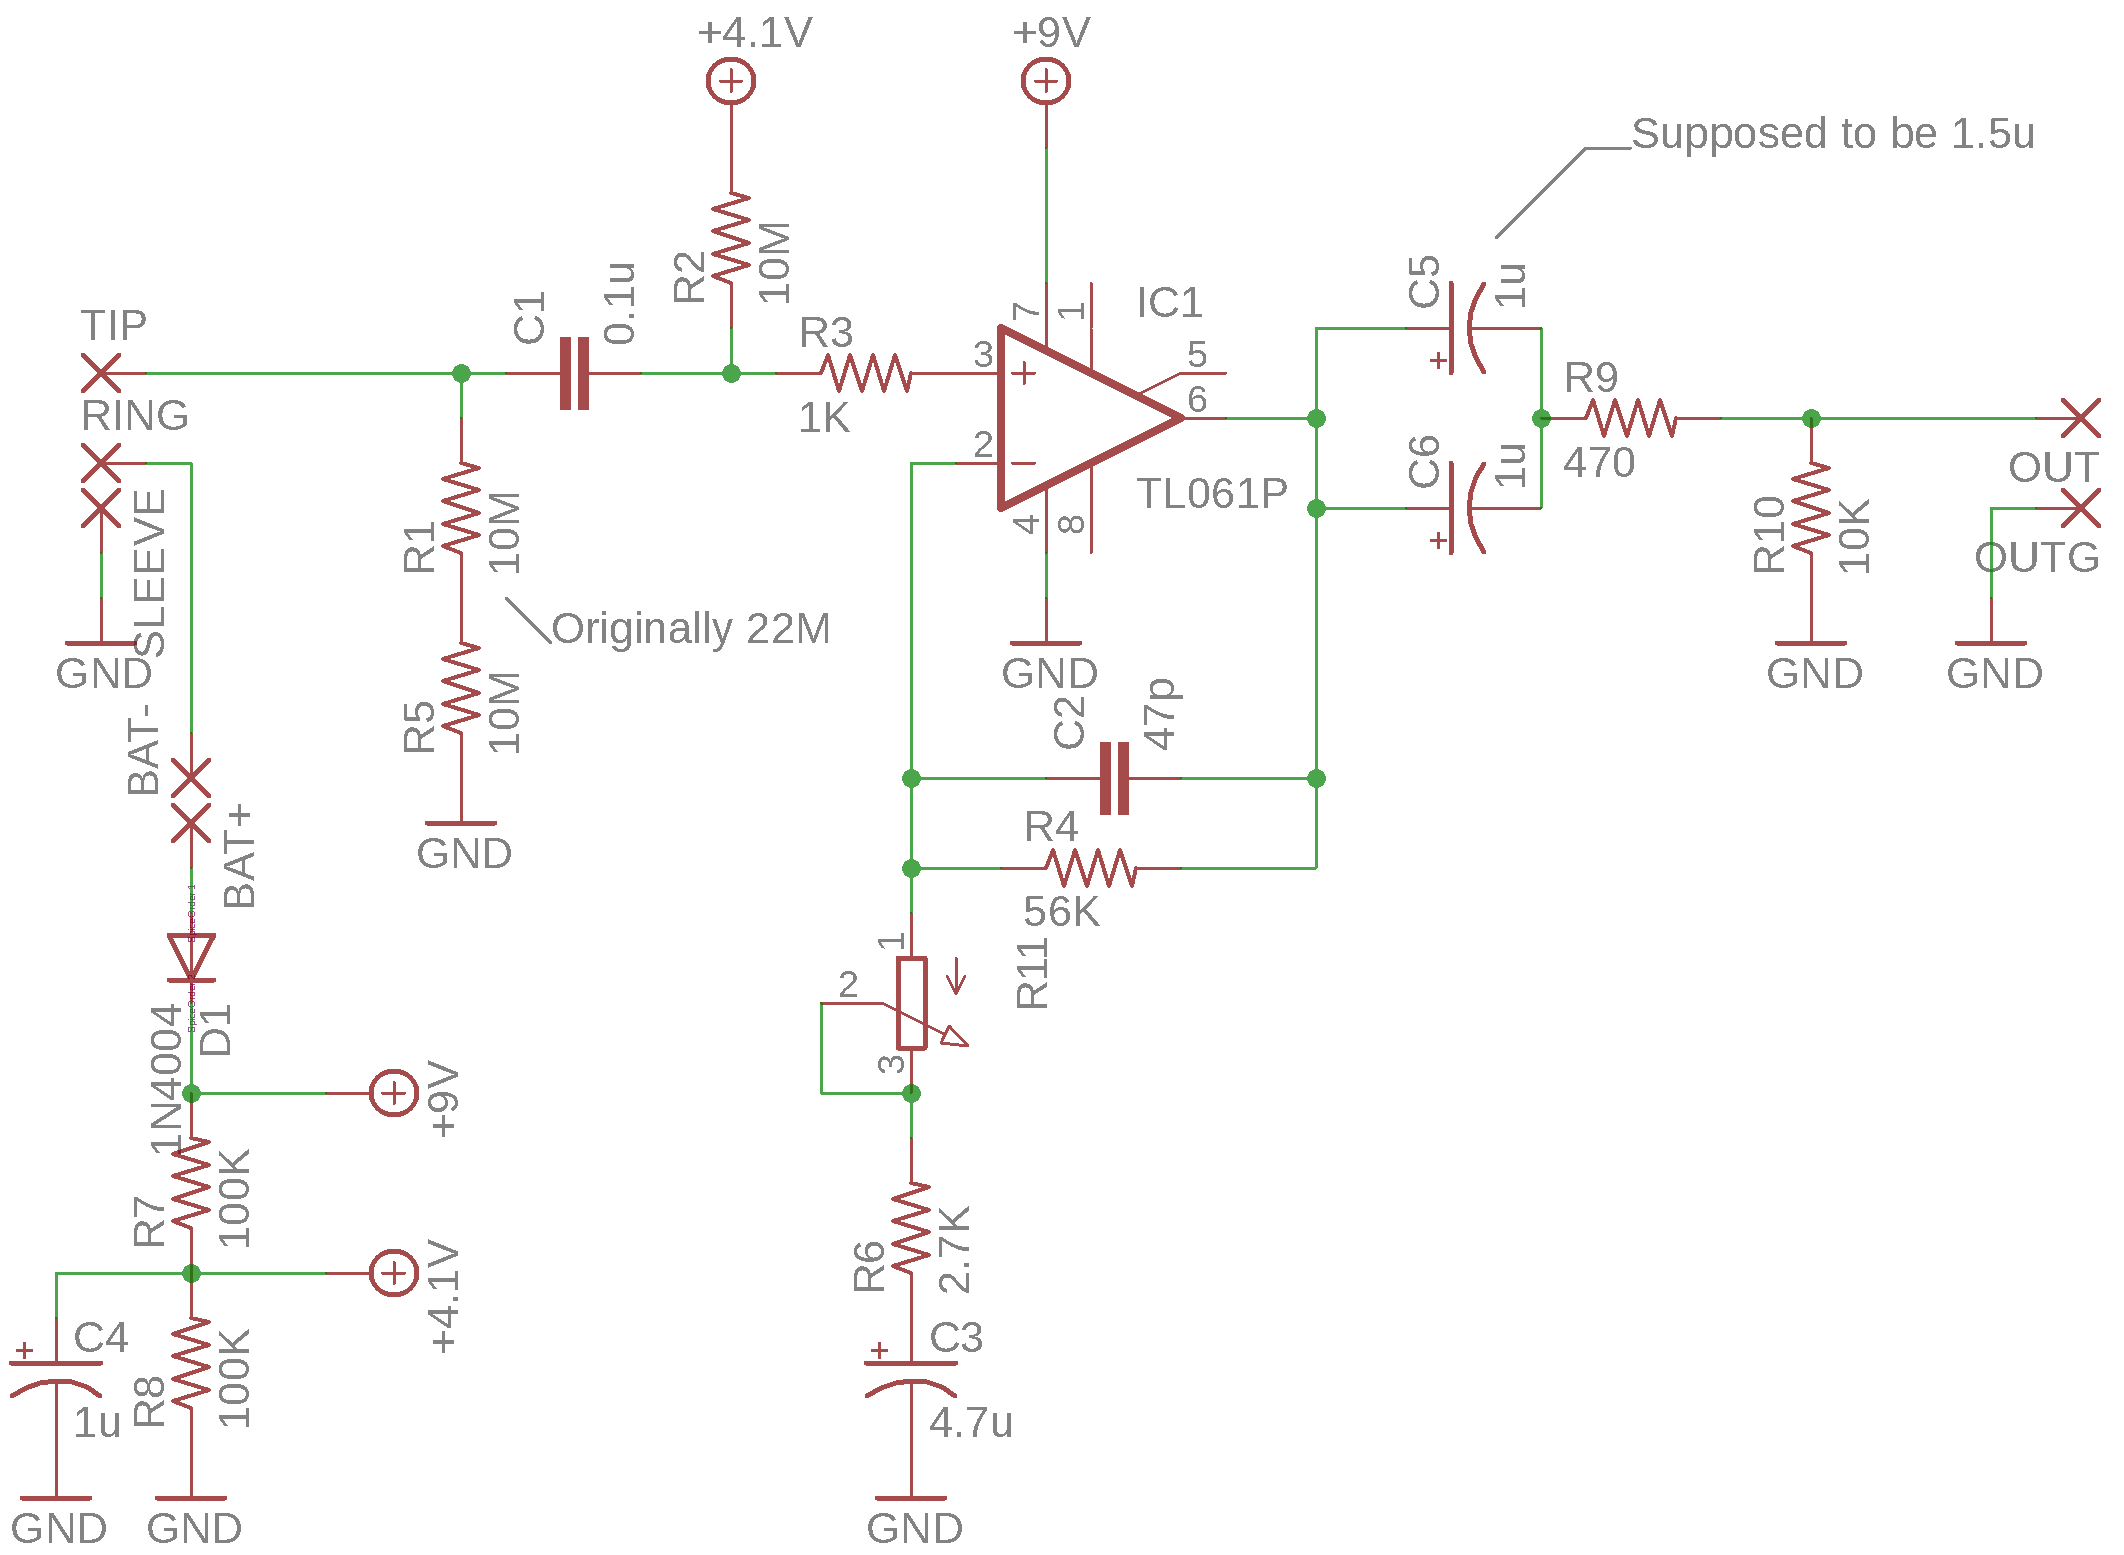
\includegraphics{img/mxr-microamp-used}
	\caption{The schematic of the assembled \textit{MXR® MICRO AMP}}
	\label{fig:mxr-microamp-used}
\end{figure}
This should not influence the frequency response in any significant manner.

\paragraph*{}
The assembled circuit was connected to a computer with sine-wave generating 
capabilities via a $3.5\si{mm}$ jack on the computer. At the output it was 
connected to an oscilloscope, which was set 
to automatically measure the data every two seconds. The recorded data was 
then copied to a computer which did the data processing. A program on the 
computer enabled the sine-wave frequency to be automatically increased by a 
fixed value of $25Hz$\footnote{Available at: 
\url{https://github.com/markovejnovic/freq-response-microamp/tree/master/src}}.

\section{Data}

\subsection{Raw data}
\paragraph*{}
The oscilloscope recorded a total of $23376000$ different voltage points for 
varying frequencies. Due to the sheer amount of raw data, it was only possible 
to publish it online and it is available at the following link:
\url{https://github.com/markovejnovic/freq-response-microamp/}.

The uncertainty is not given online, however the oscilloscope specification 
(%TODO Cite
) states that the voltage uncertainty is %TODO Figure that out

\subsection{Data processing}
\paragraph*{}
For every frequency, the oscilloscope generated $4000$ individual voltage 
points. Using a custom \textit{python}, \textit{matplotlib} and \textit{numpy} 
program\footnote{
Available at
\url{https://github.com/markovejnovic/freq-response-microamp/tree/master/src}.
}, a sinusoidal fit was achieved. An example of this is given in figure 
\ref{fig:process1-example}.
\begin{figure}[ht]
	\centering
	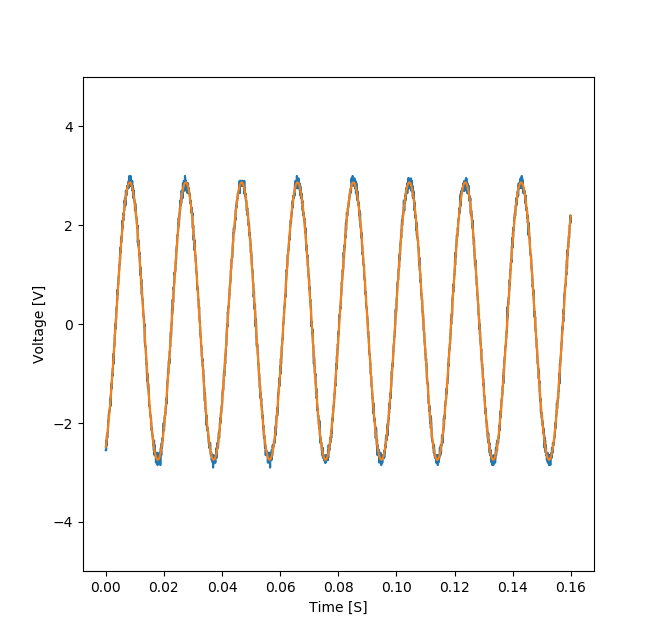
\includegraphics[width=0.8\textwidth]{img/process1-example}
	\caption{An example of plotted raw data and a sinusoidal fit with the 
	original data given in blue and the fit in orange}
	\label{fig:process1-example}
\end{figure}
From this fit the amplitude was calculated. 

\paragraph*{}
This has been achieved for all calculated frequencies. With the amplitudes 
for different frequencies present, a final graph was plotted\footnote{
Again, available at: 
\url{https://github.com/markovejnovic/freq-response-microamp/tree/master/src}}
- the relationship between the frequency and the amplitude of the signal, 
given in figure \ref{fig:freq-response-v-lin}.
\begin{figure}[ht]
	\centering
	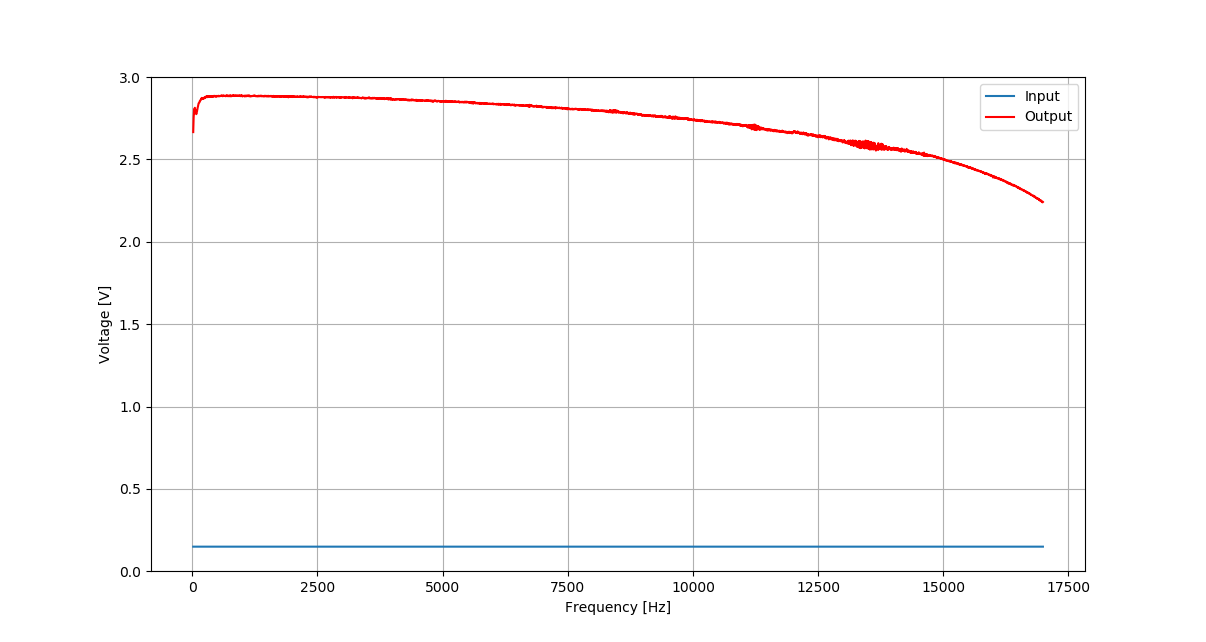
\includegraphics[width=\textwidth]{img/freq-response-v-lin}
	\caption{The relationship between the amplitude of the output voltage and 
	the frequency of an \textit{MXR® MICRO AMP}}
	\label{fig:freq-response-v-lin}
\end{figure}

\paragraph*{}
Due to human ears hearing sound in a logarithmic fashion, the logarithmic plot 
is given in figure \ref{fig:freq-response-db-log}. Notice that conversion has 
been done from absolute voltage to relative gain using the formula:
$$L = 20log_{10}\frac{V_o}{V_i} \si{dB}$$
\begin{figure}[ht]
	\centering
	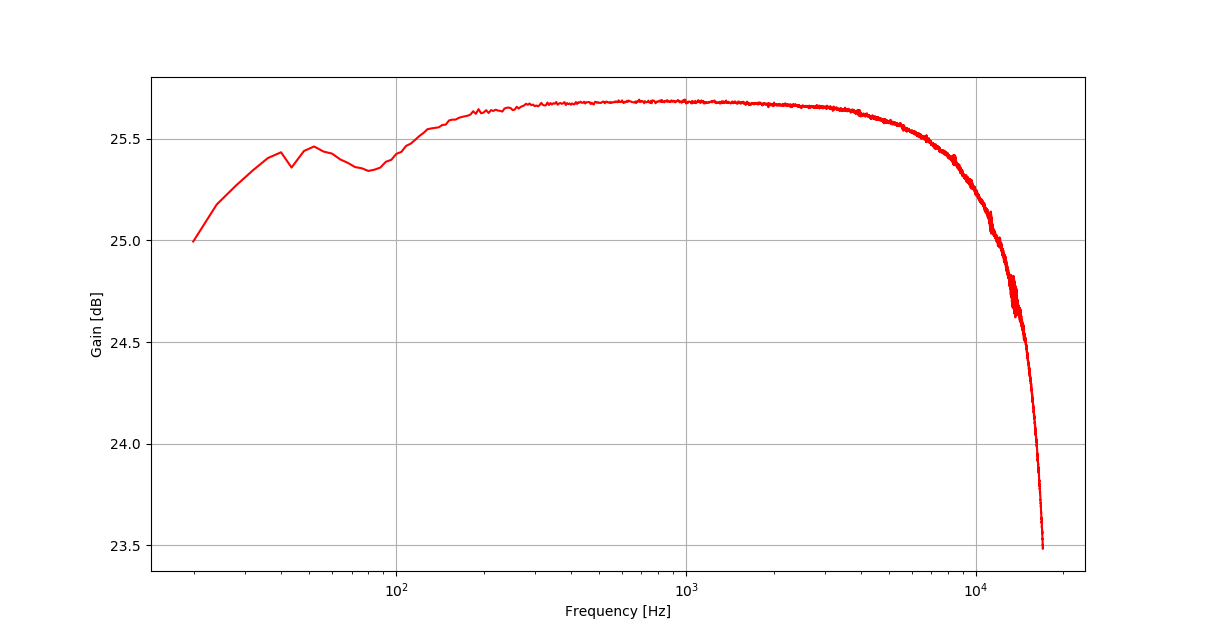
\includegraphics[width=\textwidth]{img/freq-response-db-log}
	\caption{The relationship between the frequency and the gain of the 
	\textit{MXR® MICRO AMP}}
	\label{fig:freq-response-db-log}
\end{figure}

\section{Analysis}

\subsection{Comparing to other research}
\paragraph*{}
\textit{Electrosmash.com} conducted similar research in the field, measuring 
the frequency response of the \textit{MXR® MICRO AMP}. Their results are given 
verbatim in figure \ref{fig:freq-response-db-log-electrosmash}.
\begin{figure}[ht]
	\centering
	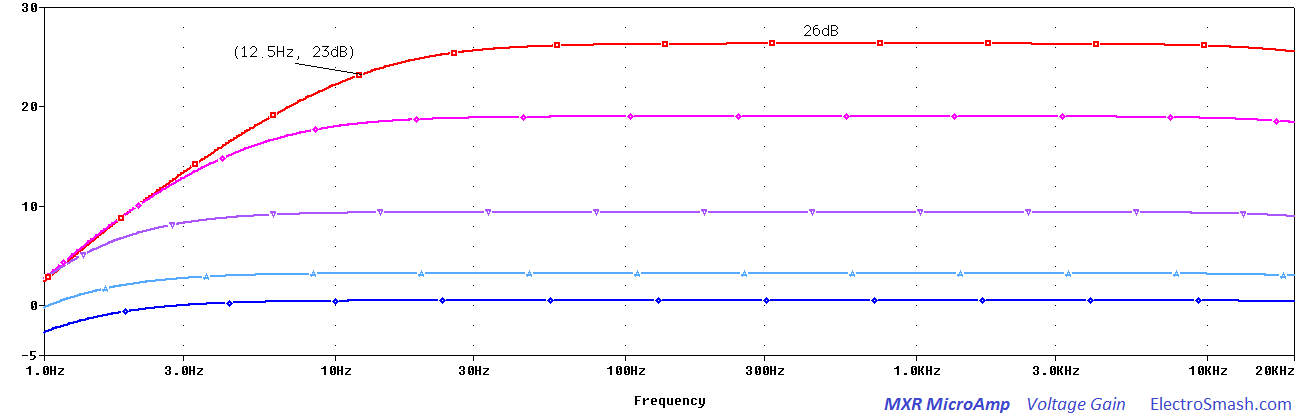
\includegraphics[width=\textwidth]{img/freq-response-db-log-electrosmash}
	\caption{The relationship between the frequency and gain of the 
	\textit{MXR® MICRO AMP} as measured by \textit{Electrosmash.com}}
	\label{fig:freq-response-db-log-electrosmash}
\end{figure}
The data they acquired differs somewhat than the one acquired in this study 
in the range of $25\si{Hz}$-$80\si{Hz}$. It is somewhat difficult to pinpoint 
the exact cause of the filtering present around $80\si{Hz}$, however, it could  
be attributed to the fact that the circuit in this research was physically 
assembled on a breadboard, which does possess some innate capacitance and 
resistance in the connections between jumper cables and the breadboard holes.

\subsection{Frequency response}
\paragraph*{}
The data indicates a non-flat frequency response. Graph 
\ref{fig:freq-response-db-log} shows that the pedal has some oscillations in 
gain between the $25\si{Hz}$ and $80\si{Hz}$ range. There is a valley at 
$80\si{Hz}$, after which the gain increases steadily, flattening out around 
$250\si{Hz}$. The amplifier's guitar response remains flat until around 
$4000\si{Hz}$. These all indicate that the pedal is designed to operate in 
the $80\si{Hz}$-$4000\si{Hz}$ frequency range. Given that a typical guitar's 
frequency range is between $80\si{Hz}$ and $1200\si{Hz}$ (Case) the pedal 
performs quite well and is sufficiently flat in the operating range.

\subsection{Other phenomena}
\paragraph*{}
While gathering the data, it was noticed that distortion occurred at 
frequencies higher than $15\si{kHz}$. Since the goal of this research was not 
investigating distortion, it was ignored, however, given that this pedal is 
not supposed to have any distortion to it, it is most likely worthwhile to 
investigate the total harmonic distortion of the pedal.

\section{Conclusion}
\paragraph*{}
Although the measurements acquired in this study are not equal to those 
of other parties, even this data indicates that the frequency response of 
the \textit{MXR® MICRO AMP} guitar pedal is sufficiently flat in the frequency 
band in which it operates.

\newpage
\section*{Works cited}
\begin{hangparas}{.25in}{1}
	Case, Alex. "Guitars". Recordingology.Com, 
	\url{http://recordingology.com/in-the-studio/guitars/}. 
	Accessed 26 July 2018.


	Horowitz, Paul, and Winfield Hill. \textit{The Art Of Electronics}. 3rd ed., 
	Cambridge, 2015.


	Hunter, John D. \textit{``Matplotlib: A 2D Graphics Environment''}. 
	Computing In Science \& Engineering, vol 9, no. 3, 2007, pp. 90-95. 
	Institute Of Electrical And Electronics Engineers (IEEE), 
	doi:10.1109/mcse.2007.55. Accessed 27 July 2018.

	
	Jim Dunlop. \textit{MXR® MICRO AMP}. 1984.


	Jones E, Oliphant E, Peterson P, et al. \textit{SciPy: Open Source 
	Scientific Tools for Python}. 2001-. \url{http://www.scipy.org/}. 
	Accessed 26 July 2018.


	"MXR Microamp Analysis". Electrosmash.com, 2018, 
	\url{https://www.electrosmash.com/mxr-microamp}. Accessed 19 July 2018.


	Python Software Foundation. \textit{Python Language Reference}, version 
	3.6. http://www.python.org


	Texas Instruments. \textit{Tl06xx Low-Power JFET-Input Operational 
	Amplifiers}. 1978.


\end{hangparas}

\end{document}

